\documentclass[a4paper]{article}

\usepackage{geometry}
\usepackage{xcolor}
\usepackage{color,soul}
\usepackage{mathrsfs}
\usepackage{tikz-cd}
\usepackage{tcolorbox}
\usepackage{amsthm}
\usepackage{amsmath}
\usepackage{amssymb}
\usepackage{fancyhdr}
\pagestyle{fancy}
\usepackage{wrapfig}
\usepackage{tabularx}
\usepackage[font={small, sf},labelfont=bf]{caption}


\usepackage{titlesec}
\titleformat{\section}[block]{\color{black}\Large\bfseries\filcenter}{}{1em}{}



\setlength{\headheight}{40pt}
\usepackage{graphicx}
\usepackage[export]{adjustbox}


\usepackage{imakeidx}
\makeindex[columns=2, title=Index, intoc]


\usepackage{hyperref}
\usepackage{cleveref}

\hypersetup{
	colorlinks=true,
	linkcolor=blue,
	filecolor=magenta,      
	urlcolor=cyan,
	pdftitle={Sharelatex Example},
	pdfpagemode=FullScreen,
}

\urlstyle{same}


\newcommand{\FHom}{\mathcal{H} o m}
\newcommand{\sheafification}{\mathcal{F}^+}
\newcommand{\Id}{\textrm{Id}}
\newcommand{\Hom}{\textrm{Hom}}
\newcommand{\Spec}{\textrm{Spec }}
\newcommand{\Sch}{\textrm{Sch}}
\newcommand{\Set}{\textrm{Set}}
\newcommand{\Grass}{\textrm{Grass}}
\newcommand{\Mod}{\textrm{Mod}}
\newcommand{\id}{\textrm{id}}
\newcommand{\Ob}{\textrm{Ob}}
\newcommand{\Ext}{\textrm{Ext}}
\newcommand{\Tor}{\textrm{Tor}}
\newcommand{\Invlim}{\lim\limits_{\longleftarrow}}
\newcommand{\Dirlim}{\lim\limits_{\longrightarrow}}
\newcommand{\Gal}{\textrm{Gal}}
\newcommand{\F}{\mathscr{F}}
\newcommand{\res}{\text{res}}
\newcommand{\primep}{\mathfrak{p}}
\newcommand{\bigo}{\mathcal{O}}
\newcommand\smallo{
	\mathchoice
	{{\scriptstyle\mathcal{O}}}% \displaystyle
	{{\scriptstyle\mathcal{O}}}% \textstyle
	{{\scriptscriptstyle\mathcal{O}}}% \scriptstyle
	{\scalebox{.7}{$\scriptscriptstyle\mathcal{O}$}}%\scriptscriptstyle
}
\newcommand{\Aut}{\textrm{Aut}}
\newcommand{\projs}{\mathbf{Proj}(S)}
\newcommand{\Proj}{\mathbf{Proj}}
\newcommand{\Ass}{\textrm{Ass}}
\newcommand{\Div}{\textrm{Div}}
\newcommand{\pdiv}{\textrm{div}}
\newcommand{\Cov}{\textrm{Cov}}
\newcommand{\Op}{\textrm{Op}}


\newtheoremstyle{theorem}{}{}{}{}{\color{blue}\bfseries}{.}{ }{}
\theoremstyle{theorem}
\newtheorem{theorem}{Theorem}[section]
\newtheorem{lemma}[theorem]{Lemma}
\newtheorem{corollary}[theorem]{Corollary}
\newtheorem{proposition}[theorem]{Proposition}

\theoremstyle{definition}
\newtheorem{definition}{Definition} [section]
\newtheorem{example}{Example}
\newtheorem{xca}[theorem]{Exercise}



\theoremstyle{remark}
\newtheorem{remark}{Remark}

\newtheoremstyle{gremark}{}{}{}{}{\color{red}\bfseries}{.}{ }{}
\theoremstyle{gremark}
\newtheorem{gremark}{Future Expansion Necessary}

\newtheoremstyle{discussion}{}{}{}{}{\color{orange}\bfseries}{.}{ }{}
\theoremstyle{discussion}
\newtheorem{discussion}{Discussion}

\newtheoremstyle{notation}{}{}{}{}{\color{orange}\bfseries}{.}{ }{}
\theoremstyle{notation}
\newtheorem{notation}{Notation}


\newtcolorbox{mybox}[3][]
{
	colframe = #2!25,
	colback  = #2!10,
	coltitle = #2!20!black,  
	#1,
}




\begin{document}
	
	
	
\section*{Example}

\begin{theorem}
	Let $A$ be an embedded $n$-manifold with boundary $\partial A$. Let $v$ be a direction such that $h_v^{A}: A \rightarrow \mathbb{R}$ is a Morse function. Let the interval	decomposition of the $k$-dimensional extended persistent homology of $h_v^{\partial A}: \partial A \rightarrow \mathbb{R}$ be
	$$
	\mathrm{XPH}_k\left(\partial A, h_v\right)=\bigoplus_{\left[b_i, d_i\right) \in S_X} \mathcal{I}_{\left[b_i, d_i\right)} .
	$$
	
	Let $J_A^k$ be the subset of intervals $\left[b_i, d_i\right)$ such that $b_i=\left(h_v(p)\right.$, ord) for some $p \in \operatorname{Crit}\left(h_v^A,(k,+1)\right)$ , or $b_i=\left(h_v(p)\right.$, rel $)$ for some $p \in \operatorname{Crit}\left(h_v^A,(n-k-1,-1)\right)$. Then
	$$
	\mathrm{XPH}_k\left(A, h_v\right)=\bigoplus_{\left[b_i, d_i\right) \in J_A^k} \mathcal{I}_{\left[b_i, d_i\right)} .
	$$
\end{theorem}

For simplicity, we will illustrate all possible critical points.

\begin{definition}
	
	For a given vertex, we have $3\times 2$ possibilities for critical points.
	
	If the figure encapsulates volume:
	If volume surrounds the figure: 
	
	\begin{figure}[ht]
		\centering
		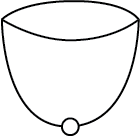
\includegraphics[scale=0.5]{minima.png}
		\caption{Index= (0,-)}
	\end{figure}

	\begin{figure}[ht]
		\centering
		
\includegraphics[scale=0.5]{maxima.png}
		\caption{Index= (0,-)}
	\end{figure}
	
	\begin{figure}[ht]
		\centering
		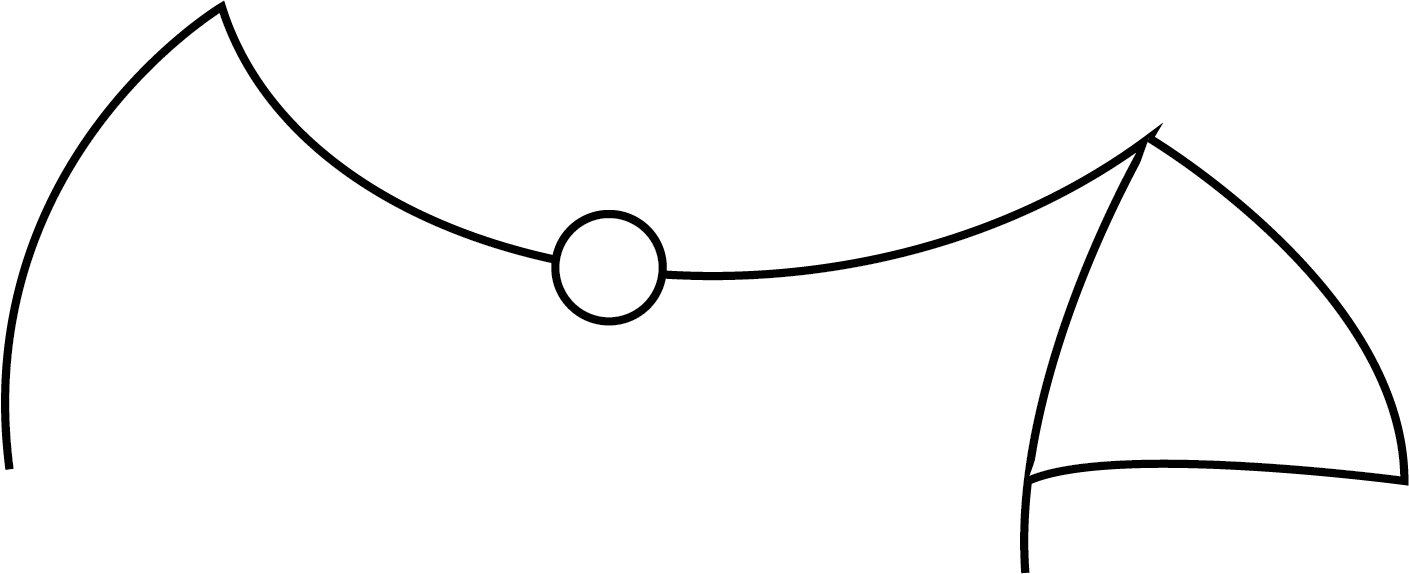
\includegraphics[scale=0.5]{saddle_point.png}
		\caption{Index= (0,-)}
	\end{figure}
	
\end{definition}

\pagebreak




	\begin{wrapfigure}[5]{R}{0.65\textwidth}
	\vspace{-1.75\baselineskip}
	\begin{tabularx}{\linewidth}{@{} cX @{}}
		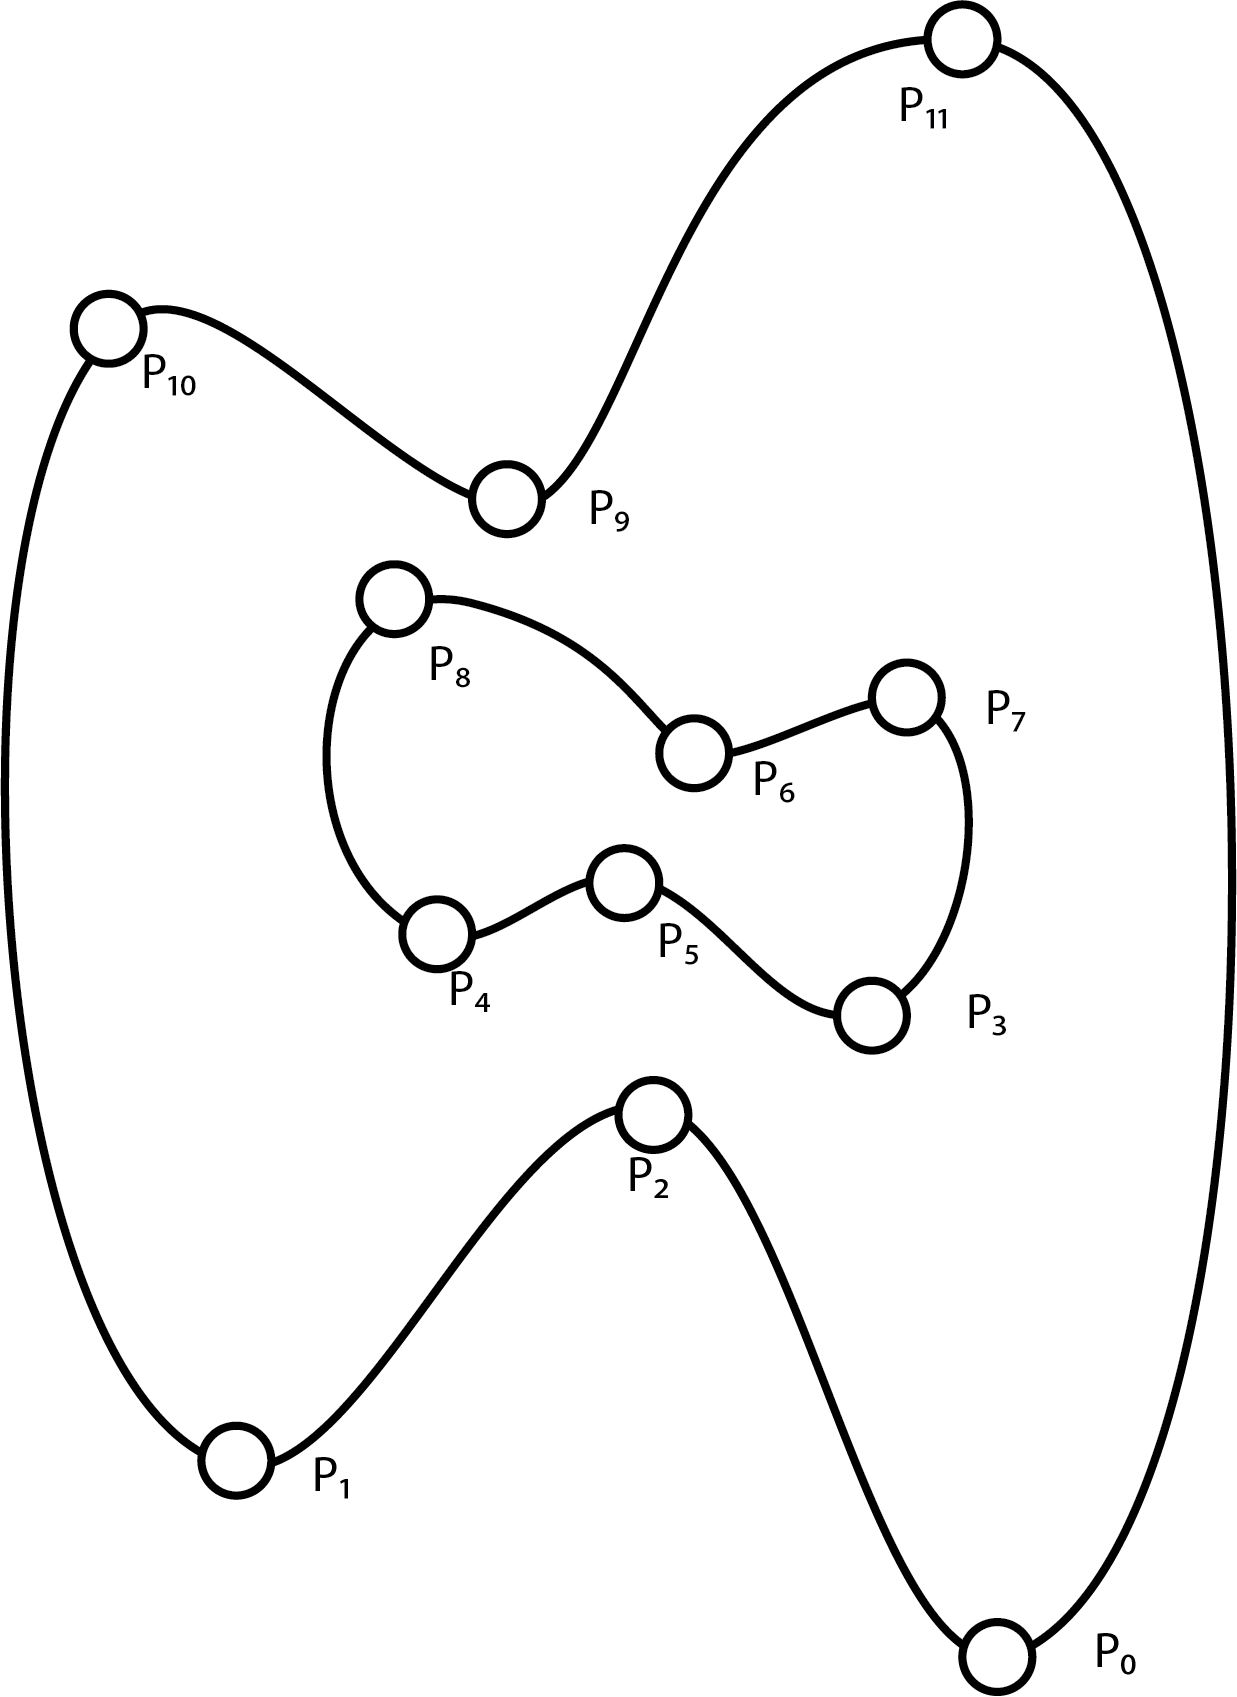
\includegraphics[scale=0.41,valign=T]{example_figure_1.png}
		&
		\caption[Wonky Torus]
		{Wonky Torus. This is a "general" slice of a torus with boundary. The circles represent critical points.}
		\label{fig:transformer3}
	\end{tabularx}
\end{wrapfigure}



It is well known what the homology groups of the torus are:
\begin{enumerate}
	\item $H_0(T)=\mathbb{Z}$
	\item $H_1(T)=\mathbb{Z}\oplus\mathbb{Z}$
	\item $H_2(T)=\mathbb{Z}$
\end{enumerate}

As for the solid torus:

\begin{enumerate}
	\item $H_0(T)=\mathbb{Z}$
	\item $H_1(T)=\mathbb{Z}$
	\item $H_2(T)=0$
\end{enumerate}



\begin{example}
	Consider Figure 1. And we will compute $\mathrm{XPH}_0$. We will also compare what is happening with the critical points with respect to both $A$ and $\partial A$.
	
	\noindent

			We will start with the boundary $\partial A$ first. 
			

			
			
		\begin{enumerate}
			\item $P_0$ is a local minimum. It creates a connected component. It is actually the global minimum.
			\item $P_1$ is another local minimum. It creates another class in $H_0$.
			\item $P_2$ This is a saddle which joins the two connected components. So we pair $(P_1,P_2)$.
			\item $P_3$ This is a saddle which looks like a handle. This forms an essential class in $H_1$.
			\item $P_4$ adds another handle which forms another class in $H_1$.
			\item $P_5$ is a local maximum whichs joins two cycles, so we pair $(P_4,P_5)$.
			\item $P_6$ is a local minimum, which starts a class in $H_0$.
			\item $P_7$ is a saddle, which joins the component, so we pair $(P_6,P_7)$.
			\item $P_8$ is a saddle, which forms an essential class in $H_1$.
			\item $P_9$ is a saddle which looks like a handle, which forms a class in $H_1$.
			\item $P_{10}$ is a local maximum, which kills a class in $H_1$, so we pair $(P_9,P_{10})$.
			\item $P_{11}$ Is a global maximum, which creates a class in $H_2$.
		\end{enumerate}


\noindent
	Let us contrast this with the solid torus with boundary $A$.
	
	\begin{enumerate}
		\item $P_0$ is a local minimum. It creates a connected component. It is actually the global minimum.
		\item $P_1$ is another local minimum. It creates another class in $H_0$.
		\item $P_2$ This is a saddle which joins the two connected components. So we pair $(P_1,P_2)$.
		\item $P_3$ Contributes nothing
		\item $P_4$ Contributes nothing
		\item $P_5$ Contributes nothing
		\item $P_6$ Creates connected component.
		\item $P_7$ Merges created component
		\item $P_8$ Creates H1 cycle
		\item $P_9$ Contributes nothing
		\item $P_{10}$ Contributes nothing
		\item $P_{11}$ Is a global maximum. Contributes nothing
	\end{enumerate} 

	$P_3$ is where things start becoming different for the solid donut and for its boundary.

	
	
	
	
	
	
	
\end{example}

\begin{figure}[ht]
	\centering
	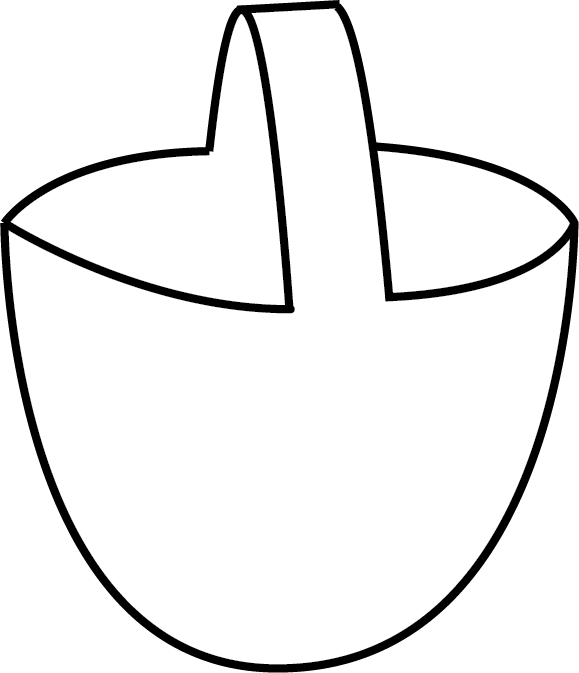
\includegraphics[scale=0.5]{handle.png}
	\caption{Handle}
\end{figure}


	
	
	\begin{theorem}
		Let $A \subset \mathbb{R}^2$ be a 2-dimensional piecewise linear manifold with boundary $X=\partial$. Fix $v \in S^1$. The 0-dimensional persistent homology of $h_v^X: X \rightarrow \mathbb{R}$ can be written as
		$$
		\mathrm{PH}_0\left(X, h_v^X\right)=\oplus_{i=1}^m \mathcal{I}_{\left[h_v\left(y_{j_i}\right), d_i\right)}
		$$
		where $y_{j_1}, \ldots y_{j_m}$ are the set of vertex representatives, and $d_1, \ldots d_m \in \mathbb{R} \cup \infty$. Here we have only included intervals with positive length.
		
		Let $J^{\text {ord }}$ be the subset of $\{1,2, \ldots m\}$ such that $d_i$ is finite and $y_{j_i}$ is (+)critical for $h_v^A$. Then
		$$
		\operatorname{Ord}_0\left(A, h_v^A\right)=\oplus_{i \in J^{\text {ord }}} \mathcal{I}_{\left[\left(h_v\left(y_{j_i}\right), \text { ord }\right),\left(d_i, \text { ord }\right)\right)}
		$$
		
		Now let $J^{\text {rel }}$ be the subset of $\{1,2, \ldots m\}$ such that $d_i$ is finite but $y_i$ is not $(+)$-critical for $h_v^A$.
		$$
		\operatorname{Rel}_1\left(A, h_v^A\right)=\oplus_{i \in J \mathrm{rel}} \mathcal{I}_{\left[\left(d_i, \mathrm{rel}\right),\left(h_v\left(y_{j_i}\right), \text { rel }\right)\right)}
		$$
	\end{theorem}
	
	\begin{theorem}
			Let $A \subset \mathbb{R}^3$ be a 3-dimensional piecewise linear manifold with boundary $\partial A$. Fix $v \in S^1$. The 0-dimensional persistent homology of $h_v^X: X \rightarrow \mathbb{R}$ can be written as
		$$
		\mathrm{PH}_0\left(X, h_v^X\right)=\oplus_{i=1}^m \mathcal{I}_{\left[h_v\left(y_{j_i}\right), d_i\right)}
		$$
		where $y_{j_1}, \ldots y_{j_m}$ are the set of vertex representatives, and $d_1, \ldots d_m \in \mathbb{R} \cup \infty$. Here we have only included intervals with positive length.
		
		Let $J^{\text {ord }}$ be the subset of $\{1,2, \ldots m\}$ such that $d_i$ is finite and $y_{j_i}$ is (+)critical for $h_v^A$. Then
		$$
		\operatorname{Ord}_0\left(A, h_v^A\right)=\oplus_{i \in J^{\text {ord }}} \mathcal{I}_{\left[\left(h_v\left(y_{j_i}\right), \text { ord }\right),\left(d_i, \text { ord }\right)\right)}
		$$
		
		Now let $J^{\text {rel }}$ be the subset of $\{1,2, \ldots m\}$ such that $d_i$ is finite but $y_i$ is not $(+)$-critical for $h_v^A$.
		$$
		\operatorname{Rel}_1\left(A, h_v^A\right)=\oplus_{i \in J \mathrm{rel}} \mathcal{I}_{\left[\left(d_i, \mathrm{rel}\right),\left(h_v\left(y_{j_i}\right), \text { rel }\right)\right)}
		$$
	\end{theorem}

	\begin{theorem}
		Proposition 4.20. Let $A \subset \mathbb{R}^n$ be an $n$-manifold with boundary $X=\partial A$. Let $v$ be a direction such that $h_v^A: A \rightarrow \mathbb{R}$ is a Morse function. Let $\left\{X_1, \ldots X_k\right\}$ be the interior boundary components of $X$ and $\left\{Y_1, \ldots Y_l\right\}$ be the exterior boundary components of $X$. Then
		$$
		\operatorname{Ess}_0\left(A, h_v\right)=\sum_{j=1}^l \mathcal{I}_{\left[\left(\min \left\{h_v\left(Y_j\right)\right\}, \operatorname{ord}\right),\left(\max \left\{h_v\left(Y_j\right)\right\}, \text { rel }\right)\right)}
		$$
		and
		$$
		\operatorname{Ess}_{n-1}\left(A, h_v\right)=\sum_{i=1}^k \mathcal{I}_{\left[\left(\max \left\{h_v\left(X_i\right)\right\}, \operatorname{ord}\right),\left(\min \left\{h_v\left(X_i\right)\right\}, \text { rel }\right)\right)}
		$$
	\end{theorem}
	
\end{document}